\section{Définitions}
\noindent\textbf{Onde plane} : Onde qui ne dépend que d'une seule variable cartésienne \\
\textbf{Onde harmonique} : Onde dont le profil est sinusoïdal ($\sim \cos, \sin$) \\
\\
\textbf{Notation} : Dans tout le cours, on notera \\
\indent $A$ : Amplitude (de la même unité que $\varphi$) \\
\indent $\omega$ : Pulsation (en rad/s) \\
\indent $\delta$ : Déphasage (en rad) \\
\indent $f$ : Fréquence (en Hz)\\
\indent $T$ : Periode temporelle \\\\
\noindent\textbf{Définition mathématique} :
On sait que $\varphi$ est une onde plane harmonique progressive si $\varphi(x,t)=f(x-ct)$ avec $f$ une fonction sinusoïdale.\\
Considérons donc qu'à l'instant $t=0$ une perturbation soit provoquée par une source sinusoïdale. On a alors :
\[\varphi(0,t)=A\cos(\omega t +\delta)\]
Avec, par définition, $\omega=2\pi f$ et $f=T^{-1}$\\
On peut alors écrire : \[\varphi(0,t)=A\cos(2\pi f+\delta)=A\cos(\frac{2\pi t}{T}+\delta)\] 
Or, la perturbation qui a lieu en $t=0$ a lieu également un instant plus tard $t+\Delta t$ en $x$ (phénomène de propagation à la celerité $c$) :
\[\varphi(x,t+\Delta t)=\varphi(0,t)=A\cos(\frac{2\pi t}{T}+\delta)\]
D'où :
\[
\varphi(x,t)=\varphi(0,t-\Delta t)=A\cos(2\pi(\frac{t-\Delta t}{T})+\delta)=A\cos(2\pi(\frac{t}{T}-\frac{c\Delta t}{cT})+\delta)=
A\cos(2\pi(\frac{t}{T}-\frac{x}{cT})+\delta)
\]
En posant $\lambda=cT$ la longueur d'onde, on a :
\[\varphi(x,t)=A\cos(2\pi(\frac{t}{T}-\frac{x}{\lambda}))\]
On pose également $k=\frac{2\pi}{\lambda}=\frac{\omega}{c}$\\
\quadri{8}
\[\forall t,x\in \mathbb{R}, n\in\mathbb{N}, \varphi(x+n\lambda,t)=\varphi(x,t)\]
\quadri{8}
\[\forall t,x\in \mathbb{R}, n\in\mathbb{N}, \varphi(x,t+nT)=\varphi(x,t)\]

\section{Equation d'Helmotz}
Etant donné notre connaissance de la forme général des ondes planes harmoniques, on peut simplifier l'équation d'onde les concernant, en effet :
\[
\left \{
  \begin{array}{ll}
  \Delta\varphi-\frac{1}{c^2}\frac{\partial^2\varphi}{\partial t^2}=0 \\
  \varphi(x,t)=A\cos(\omega t -kx+\delta) \\
  \end{array}
\right.
\Rightarrow
\left \{
  \begin{array}{ll}
  \Delta\varphi-\frac{1}{c^2}\frac{\partial^2\varphi}{\partial t^2}=0 \\
  \frac{\partial\varphi}{\partial t}=-A\omega\sin(\omega t -kx)
  \end{array}
\right.
\Rightarrow
\left \{
  \begin{array}{ll}
  \Delta\varphi-\frac{1}{c^2}\frac{\partial^2\varphi}{\partial t^2}=0 \\
  \frac{\partial^2\varphi}{\partial t^2}=-A\omega^2\cos(\omega t -kx)=-\omega^2\varphi(x,t)
  \end{array}
\right.
\]
On a alors : 
\[ \Delta\varphi+\frac{\omega^2}{c^2}\varphi = 0 \Leftrightarrow \Delta\varphi+k^2\varphi = 0 \]
Cette équation est appelée "équation d'Helmotz".

\section{Direction quelconque}
Jusqu'ici, les ondes se propageaient selon l'axe $\vec{e_x}$. Pour une direction quelconque, on introduit le vecteur d'onde $\vec{k}=k\vec{n}$ où $\vec{n}$ est dans la direction de propagation de l'onde ($\mid\mid\vec{n}\mid\mid=1$).\\
Ceci permet d'écrire pour $\vec{r}=\vec{OM}$ (fixe) : 
\[\varphi(\vec{r},t)=A\cos(\omega t -\vec{k}.\vec{r})\]
On a, par ailleurs, la relation suivante, appelée relation de dispertion : $\vec{k}^2=k^2$

\section{Représentation}

\noindent\textbf{Représentation en 1D} :
\begin{center}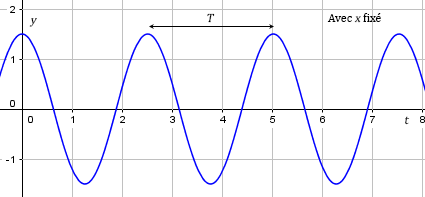
\includegraphics[width=8cm]{img/periode_T.png}\end{center}
\textbf{Représentation en 2D} :
\begin{center}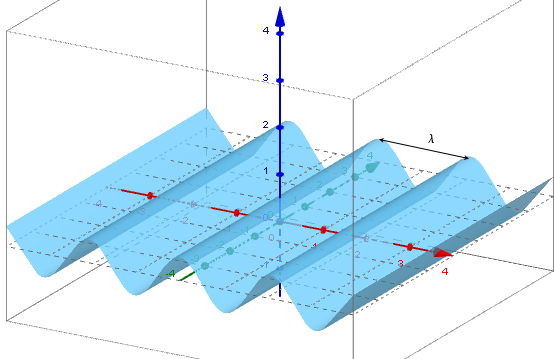
\includegraphics[width=8cm]{img/onde_2D.png}\end{center}
\textbf{Représentation en 3D} :
\begin{center}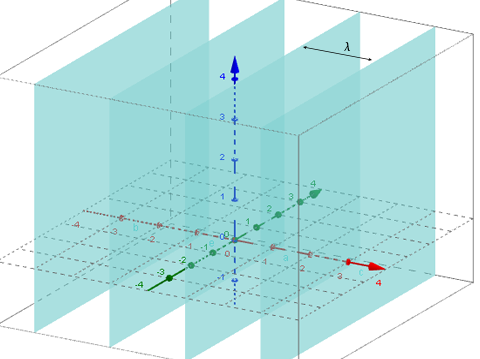
\includegraphics[width=8cm]{img/onde_3D.png}\end{center}

\section{Exemples d'ondes planes harmoniques}

\subsection{Ondes électromagnétiques}

\noindent\textbf{Célérité} : \\
Le champ électromagnétique $\vec{E}$ vérifie l'équation d'onde 
\[\Delta E-\frac{1}{c^2}\frac{\partial^2E}{\partial t^2}=0\]
Pour étudier la propagation des ondes électromagnétiques, on se place en dehors de la source ($\vec{j}=0$ et $\rho=0$). Les équations de Maxwell donnent alors :
\[
\left \{
  \begin{array}{l}
  \textrm{div }\vec{E}=0 \\
  \textrm{div }\vec{B}=0
  \end{array}
\right.
\textrm{ et }
\left \{
  \begin{array}{l}
  \vec{\textrm{rot }}\vec{E}=-\frac{\partial{\vec{B}}}{\partial t} \\
  \vec{\textrm{rot }}\vec{B}=\mu_0\varepsilon_0\frac{\partial\vec{E}}{\partial t}
  \end{array}
\right.
\]
Or : \[\Delta\vec{E}=\vec{\textrm{grad }}\textrm{div }\vec{E}-\vec{\textrm{rot }}\vec{\textrm{rot }}\vec{E}=-\vec{\textrm{rot }}\vec{\textrm{rot }}\vec{E}\] (car $\textrm{div }\vec{E} = 0$)\\
D'autre part : \[\frac{\partial^2\vec{E}}{\partial t^2}=\frac{\partial}{\partial t}(\frac{\partial\vec{E}}{\partial t})=\frac{\partial}{\partial t}(\frac{1}{\mu_0\varepsilon_0}\vec{\textrm{rot }}\vec{B})=\frac{1}{\mu_0\varepsilon_0}\vec{\textrm{rot }}\frac{\partial \vec{B}}{\partial t}=-\frac{1}{\mu_0\varepsilon_0}\vec{\textrm{rot }}\vec{\textrm{rot }}\vec{E}\]
D'où :
\[
\left \{
  \begin{array}{l}
  \Delta\vec E - \mu_0\varepsilon_0\frac{\partial^2\vec E}{\partial t^2}=0\\
  \Delta\vec E - \frac{1}{c^2}\frac{\partial^2\vec E}{\partial t^2}=0
  \end{array}
\right.
\Rightarrow c = \sqrt{\frac{1}{\mu_0\varepsilon_0}}
\]
\quadri{5}

\noindent\textbf{Spectre electromagnétique} : \\
\quadri{11}

\noindent\textbf{Orientation de $\vec k, \vec E$ et $\vec B$} : \\
\quadri{8}

\noindent\textbf{Energies et Puissance}
\[ U=\frac{1}{2}\varepsilon_0E^2+\frac{1}{2}\mu_0B^2 \]
\[ \vec p=\frac{1}{\mu_0}\vec E \wedge \vec B \]
On note également la vitesse d'énergie comme étant : $v_{energie}=\frac{\mid\mid\vec p\mid\mid}{U}=c$ \\
\emph{Remarque} : Pour le soleil, $p=1,4.10^3$ W/m$^3$.

\subsection{Ondes transversales dans une corde}

\quadri{10}
On a : $dF_y=\tau'_y-\tau_y=\tau\sin\alpha'-\tau\sin\alpha\approx\tau(\alpha'-\alpha)=\tau d\alpha=\tau\frac{\partial\alpha}{\partial x}dx$\\
De plus, $\alpha \approx\tan\alpha=\frac{\partial\varphi}{\partial x}$. D'où, $dF_y=\tau\frac{\partial \alpha}{\partial x}dx=\frac{\partial^2 \varphi}{\partial x^2}dx$. \\ \\
\textbf{PFD} : $\sum F=m\gamma \Rightarrow dF_y=dm \frac{\partial^2\varphi}{\partial t^2}$ avec $dm=\frac{M}{L}dx=\rho_Ldx$ ($\rho_L$ : masse linéique). Ou encore : $dF_y=\rho_L\frac{\partial^2\varphi}{\partial t^2}dx$. \\\\
On a alors :
\[
\left \{
  \begin{array}{l}
  dF_y=\rho_L\frac{\partial^2\varphi}{\partial t^2}dx \\
  dF_y=\tau\frac{\partial^2\varphi}{\partial x^2}dx 
  \end{array}
\right.
\Rightarrow \Delta\varphi - \frac{\rho_L}{\tau}\frac{\partial^2\varphi}{\partial t^2}=0
\Rightarrow c = \sqrt{\frac{\tau}{\rho_L}}
\]

\subsection{Ondes sonores (longitudinales)}

\noindent On se place dans un milieu où règnent les champs :\\
\indent Pression : $p_T(M,t)=p_0+p(M,t)$ ($p<<p_0$)\\
\indent Masse volumique : $\rho_T(M,t)=\rho_0+\rho(M,t)$ ($\rho<<\rho_0$)\\
\indent Vitesse des particules d'air : $v_T(M,t)=v_0+v(M,t)$ ($v_0=0$ ici)\\\\
Les constantes $p_0, \rho_0$ représentent la pression et la masse volumique du milieu "au repos". Les fonctions $p,v$ et $\rho$ représentent la perturbation dans ce milieu.
\quadri{8}
On approxime classiquement $\xi(x+dx)\approx\xi(x)+d\xi$.\\\\
Nous allons établir trois équations liées au problème : l'équation d'état, l'équation de conservation de la masse volumique, et le PFD sur l'élement de surface $S$.\\

\noindent\textbf{Equation d'état}\\

On introduit tout d'abord une nouvelle quantité appelée "Module de compressibilité" (en Pascal) dont on se servira plus tard : \[\kappa=\rho_0\frac{\partial p}{\partial \rho}\]
La pression est fonction de la masse volumique, donc on peut écrire $p_T=f(\rho_T)$ (avec $p_0=f(\rho_0)$). Etant donné que $\rho$ est petit devant $\rho_0$, on peut appliquer les formules de Taylor sur $f$ :
\[p_T=f(\rho_T)=f(\rho_0+\rho)\approx f(\rho_0)+\rho\frac{\partial f}{\partial \rho}(\rho_0)=p_0+\rho\frac{\partial p}{\partial \rho}(\rho_0)\]
Or, $p=p_T-p_0$. On trouve alors l'équation d'état :
\[p=\rho\frac{\kappa}{\rho_0}\]

\noindent\textbf{Equation de conservation de la masse}

La masse élémentaire est à tout instant $dm=\rho_TdV$, où $dV$ est un volume élementaire.\\
En particulier :
\[
\left \{
\begin{array}{ll}
\textrm{Avant la perturbation :} & dm = \rho_0Sdx \\
\textrm{Pendant la perturbation :} & dm = \rho_TS(dx+d\xi)
\end{array}
\right.
\]
En approximant $d\xi\approx \frac{\partial\xi}{\partial x}dx$, la conservation de la masse volumique avant et pendant la perturbation s'écrit :
\[
\begin{array}{ll}
 & \rho_0Sdx = \rho_TS(dx+\frac{\partial\xi}{\partial x}dx)\\
\Rightarrow & \rho_0Sdx=\rho_TSdx(1+\frac{\partial\xi}{\partial x})\\
\Rightarrow & \rho_0=\rho_T(1+\frac{\partial\xi}{\partial x}) \\
\Rightarrow & \rho_T=\rho_0(1+\frac{\partial\xi}{\partial x})^{-1} \\
\Rightarrow & \rho_T=\rho_0(1-\frac{\partial\xi}{\partial x}) \textrm{ car } \frac{\partial\xi}{\partial x} << 1
\end{array}
\]

\noindent\textbf{Equation du PFD} : équation d'Euler

Bilan des forces : Pressions $F(x,t)$ à gauche, pression $F(x+dx,t)$ à droite.
\[
\begin{array}{ll}
& \sum F_{ext} = dm\gamma \\
\Rightarrow & F(x)-F(x+dx) = dm\gamma \\
\Rightarrow & p_T(x,t)S-p_T(x+dx, t)S=\rho_TdV\frac{\partial^2\xi}{\partial t^2} \\
\Rightarrow & p_T(x,t)S-p_T(x,t)S-dx\frac{\partial p_T}{\partial x}S=\rho_TSdx\frac{\partial^2\xi}{\partial t^2} \\
\Rightarrow & \frac{\partial p_T}{\partial x}=-\rho_T\frac{\partial^2\xi}{\partial t^2}
\end{array}
\]

\noindent\textbf{Résolution}

\noindent On a donc : 
\[
\left \{
\begin{array}{ll}
p=\rho\frac{\kappa}{\rho_0} & (1) \\
\rho_T=\rho_0(1-\frac{\partial\xi}{\partial x}) & (2) \\
\frac{\partial p_T}{\partial x} = -\rho_T\frac{\partial^2\xi}{\partial t^2} & (3)
\end{array}
\right.
\]
L'équation $(2)$ donne 
\[\rho_T-\rho_0=-\rho_0\frac{\partial \xi}{\partial x} \Rightarrow \frac{\rho_T-\rho_0}{\rho_0}=-\frac{\partial\xi}{\partial x}
\Rightarrow \frac{\rho}{\rho_0}=-\frac{\partial\xi}{\partial x}\]
D'où, dans $(1)$, \[p=\frac{\rho}{\rho_0}\kappa=-\kappa\frac{\partial\xi}{\partial x}\]
Enfin,
\[
\begin{array}{ll}
\frac{\partial p_T}{\partial x}=-\rho_T\frac{\partial^2\xi}{\partial t^2} & 
\Leftrightarrow \frac{\partial(p_0+p)}{\partial x}=-\rho_T\frac{\partial^2\xi}{\partial t^2} \\
& \Leftrightarrow -\kappa\frac{\partial^2\xi}{\partial x^2}=-\rho_T\frac{\partial^2\xi}{\partial t^2} \\
& \Leftrightarrow \Delta\xi-\frac{\rho_T}{\kappa}\frac{\partial^2\xi}{\partial t^2}=0
\end{array}
\]
Et par identification dans l'équation des ondes: 
\[c=\sqrt{\frac{\kappa}{\rho}}=\sqrt{\gamma R_s T_0} \textrm{  Dans l'air :  }c = 20\sqrt{273+T^C}  \]

\noindent\textbf{Impédance accoustique}

Pour la commodité des calculs, on pose $\alpha=t-\frac{x}{c}$, on a alors : $\xi(x,t)=f(\alpha)$ et :
\[
\left \{
\begin{array}{l}
p=-\kappa\frac{\partial \xi}{\partial x}=-\kappa\frac{\partial\xi}{\partial\alpha}\frac{\partial\alpha}{\partial x}=\frac{\kappa}{c_0}f'(\alpha) \\
v=\frac{\partial\xi}{\partial t} = \frac{\partial\xi}{\partial\alpha}\frac{\partial\alpha}{\partial t} = f'(\alpha)
\end{array}
\right.
\]
On a alors : \[p=\frac{\kappa}{c_0}v=\rho_0c_0v\]
On appelle "impédance accoustique" le rapport : $Z(x,t)=\frac{p(x,t)}{v(x,t)}$\\\\
\emph{Remarque} : Pour une onde plane progressive on a toujours : $Z=\rho_0c_0$\\
Pour l'air : \\
Pour l'eau : \\
\\
\emph{Remarque} : L'équation "$p(x,t)=-\kappa\frac{\partial\xi}{\partial x}$" met en évidence la quadrature de phase entre $p$ et $\xi$ ($\delta=\pi/2$).\\

\noindent\textbf{Energies}

\noindent Densité volumique d'énergie :
\[ U(x,t)=\frac{\rho_0}{2}(\frac{p^2}{Z^2}+v^2) \]
\[\bar{U}=\frac{\rho_0}{2}(\frac{\bar{p^2}}{Z^2}+\bar{v^2)} \]

\noindent Flux de puissance accoustique :
\[F(t)=pv\]
\noindent On appelle intensité accoustique, la valeur moyenne :
\[I=\bar{F}=\bar{pv}\]

\noindent\textbf{Niveau accoustique}

La définition du niveau accoustique se fait à l'aide de la pression effective définit comme la moyenne de la pression au carré. En anglais, et souvent en accoustique, on la note $p_{RMS}$, pour \emph{Root Mean Square}, car elle est égale à 
\[p_{eff}=p_{RMS}=\sqrt{\bar{p^2}}=\frac{p}{\sqrt{2}}\]
On introduit alors le niveau de pression accoustique comme (en dB) :
\[ L_p=10\log(\frac{p^2_{RMS}}{p^2_{ref}}) \]
Et le niveau d'intensité accoustique (en dB) :
\[ L_I=10\log(\frac{I}{I_{ref}})  \]

\noindent\textbf{Composition de niveaux}

Soient deux machines $M_1$ et $M_2$ émettant des ondes sonores :
\[
\begin{array}{l}
M_1 \rightarrow L_{p_1}=10\log(\frac{p_1^2}{p^2_{ref}}) \\
M_2 \rightarrow L_{p_2}=10\log(\frac{p_2^2}{p^2_{ref}})
\end{array}
\]

Si les deux machines émettent des ondes de fréquences différentes ou un spectre large voir un bruit blanc (i.e. toutes les fréquences sonores), alors le niveau sonnore résultant est :
\[ L_{p_{1+2}}=10\log(\frac{p_1^2+p_2^2}{p^2_{ref}}) \]
Sinon, le niveau sonnore résultant est :
\[ L_{p_{1+2}}=\max(L_{p_1}, L_{p_2})+\Delta L \]
Où $\Delta L$ est fonction de la différence des niveaux :

\begin{center}
\begin{tabular}{c|c}
$\mid L_{p_1}-L_{p_2}\mid$ & $\Delta L$ \\
\hline
0 - 1  & 3 dB \\
2 - 3  & 2 dB \\
4 - 9  & 1 dB \\
> 10 & 0 dB
\end{tabular}
\end{center}

\subsection{Ondes dans un barreau élastique}

\noindent\textbf{Introduction}

\quadri{7}

On appelle $\tau$ la "contrainte" et :
\[\tau=\frac{F}{S}\]

La loi de Hooke (élastique linéaire) dit que, lors d'une traction, $\Delta L \propto F$. D'où :
\[ \tau = \frac{\Delta L}{L} \]

\noindent\textbf{Ondes}

L'étude des ondes dans un barreau élastique est similaire à celle des ondes sonores où l'on remplace la pression $p$ par la contrainte $\tau$ et le module de compressibilité $\kappa$ par le module d'Young $E$. D'où, en notant $\xi$ le déplacement :
\[ \tau = -E\frac{\partial \xi}{\partial x} \]
Et avec des développements analogues à la partie précedente :
\[ \Delta\xi-\frac{\rho}{E}\frac{\partial^2\xi}{\partial t^2}=0 \Rightarrow c=\sqrt{\frac{E}{\rho}} \]
\emph{Remarque } : Les ondes de compressions, qui sont longitudinales, ne sont pas les seules existantes dans un barreau. Il peut exister également une onde transversalle dite de cisaillement et, en notant $G$ le module de cisaillement : $c_T=\sqrt{G/\rho}$

